\chapter{Design Pattern}
L'obiettivo di un design pattern è individuare gli aspetti della tua applicazione che variano e distinguerli da quelli che rimangono invariati. Questo è possibile programmando delle \textbf{interfaccie} e non delle implementazioni.
Esistono diversi tipi di design pattern:

\begin{figure}[!htb]
    \centering
    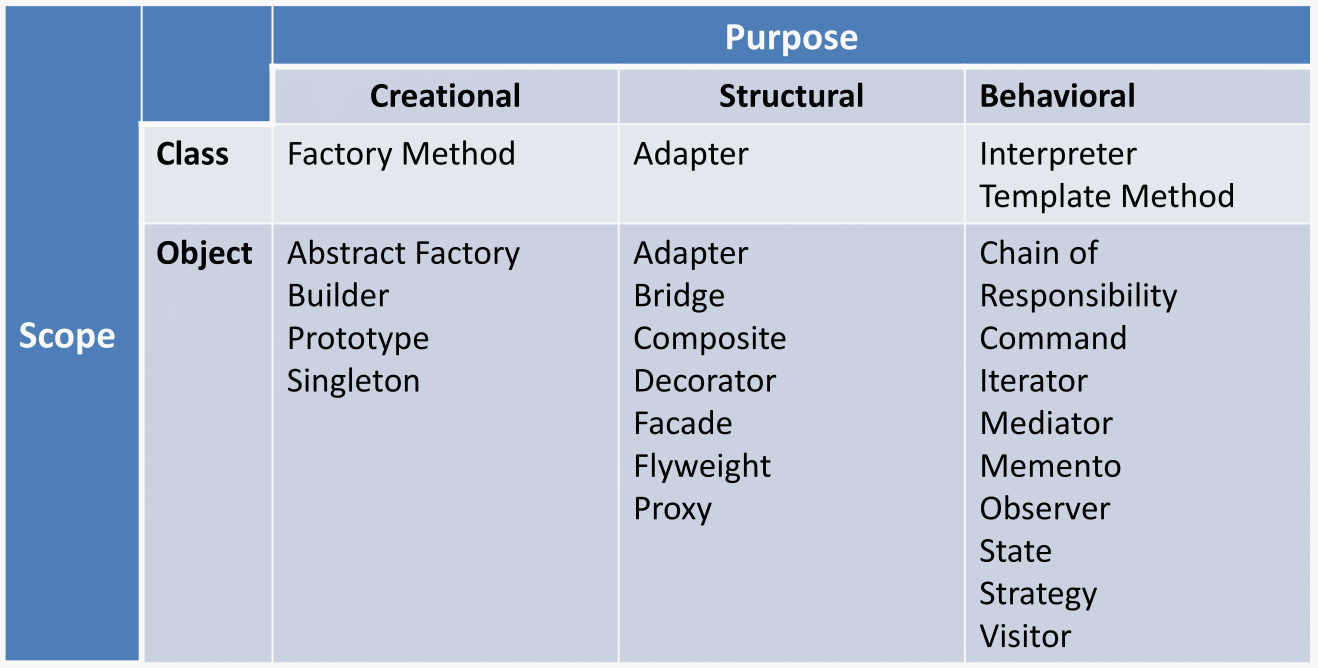
\includegraphics[width=0.7\linewidth]{Images/design_pattern/DesignTable.png}
    \caption{Classificazione dei design pattern.}
\end{figure}

\newpage
\section{Strategy Pattern}
Definisci una famiglia di algoritmi, incapsula ciascuno di essi e rendili intercambiabili. Strategy consente all'algoritmo di variare indipendentemente dai client che lo utilizzano.

\begin{boxDef}
\textcolor{brown}{Applicabilità:}
\begin{itemize}
    \item Molte classi correlate differiscono solo nel loro comportamento.
    \item Hai bisogno di diverse varianti di un algoritmo.
    \item Un algoritmo utilizza dati che i clienti non dovrebbero conoscere.
    \item Una classe definisce molti comportamenti, che si manifestano come molteplici istruzioni condizionali nelle sue operazioni.
\end{itemize}
\textcolor{brown}{Conseguenze:}
\begin{itemize}
    \item Famiglie di algoritmi collegati.
    \item Alternativa a sottoclassi.
    \item Rimozione degli statement condizionali.
    \item Overhead sulla comunicazione fra Strategy e Context.
    \item Numero elevato di oggetti.
\end{itemize}

\end{boxDef}

\begin{figure}[!htb]
    \centering
    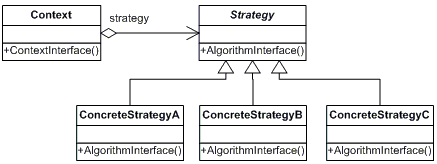
\includegraphics[width=0.7\linewidth]{Images/design_pattern/Strategy.png}
    \caption{Struttura del design pattern Strategy.}
\end{figure}

Dove:
\begin{itemize}
    \item \textbf{Strategy:} dichiara un'interfaccia comune a tutti gli algoritmi supportati. Il \textbf{context} utilizza questa interfaccia per richiamare l'algoritmo definito da una \textbf{ConcreteStrategy}.
    \item \textbf{ConcreteStrategy:} implementa l'algoritmo utilizzando l'interfaccia Strategy.
    \item \textbf{Context:} È configurato con un oggetto ConcreteStrategy. Mantiene un riferimento a un oggetto Strategy. Può definire un'interfaccia che consente a Strategy di accedere ai suoi dati.
\end{itemize}

\newpage
\section{Observer Pattern}
Si tratta di un pattern che tiene informati i tuoi oggetti quando accade qualcosa che potrebbe interessarli.
Utilizza un meccanismo \textbf{Pubblisher-Subscriber}. Un'entità pubblica informazioni, un'altra entità, che si iscrive, riceve autamaticamente le informazioni. Nel momento che non vuole più riceverne, può disiscriversi.

\begin{boxDef}
\textcolor{brown}{Applicabilità:}
\begin{itemize}
    \item Quando un'astrazione ha due aspetti, uno dipendente dall'altro.
    \item Quando una modifica a un oggetto richiede la modifica di altri oggetti e non si sa quanti oggetti debbano essere modificati.
    \item Quando un oggetto dovrebbe essere in grado di notificare altri oggetti senza fare supposizioni sull'identità di questi oggetti.
\end{itemize}
\textcolor{brown}{Conseguenze:}
\begin{itemize}
    \item Accoppiamento astratto tra soggetto e osservatore.
    \item Supporto per le comunicazioni broadcast.
    \item Aggiornamenti imprevisti.
\end{itemize}

\end{boxDef}

\begin{figure}[!htb]
    \centering
    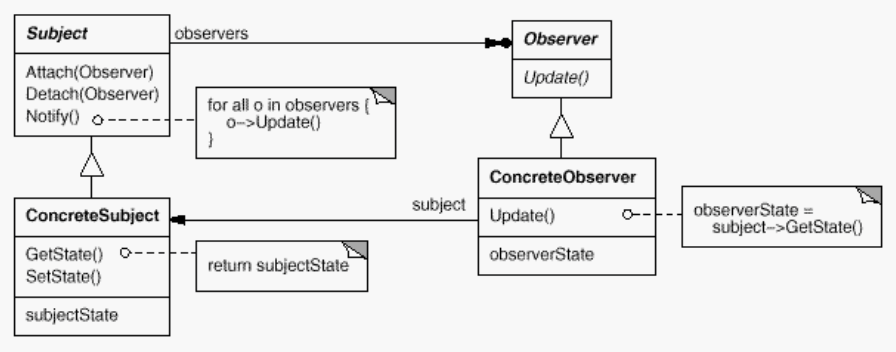
\includegraphics[width=0.7\linewidth]{Images/design_pattern/Observer.png}
    \caption{Struttura del design pattern Observer.}
\end{figure}

Dove:
\begin{itemize}
    \item \textbf{Subject:} conosce tutti i suoi \textbf{observer}. Ogni observer può avere un soggetto da osservare, tramite le funzione di \textbf{detach} e \textbf{attach} di ogni soggetto.
    \item \textbf{Observer:} interfaccia di aggiornamento per gli oggetti che devono essere notificati delle modifiche a un soggetto.
    \item \textbf{ConcreteSubject:} memorizza lo stato di interesse degli oggetti \textbf{ConcreteObserver} e invia una notifica ai suoi osservatori quando il suo stato cambia.
    \item \textbf{ConcreteObserver:} implementa l'interfaccia \textbf{Observer}.
\end{itemize}


\newpage
\section{Decorator Pattern}
I decoratori hanno lo stesso supertipo degli oggetti che decorano, possiamo passare un oggetto decorato al posto dell'oggetto originale.
Il decoratore aggiunge il proprio comportamento prima e/o dopo aver delegato all'oggetto decorato il resto del lavoro. Gli oggetti possono essere decorati in qualsiasi momento, quindi possiamo decorarli dinamicamente in fase di esecuzione con tutti i decoratori che desideriamo.

\begin{boxDef}
\textcolor{brown}{Applicabilità:}
\begin{itemize}
    \item Per aggiungere responsabilità ai singoli oggetti in modo dinamico e trasparente, ovvero senza influenzare altri oggetti.
    \item Per responsabilità che possono essere revocate.
    \item Quando l'estensione tramite sottoclassi non è praticabile.
\end{itemize}
\textcolor{brown}{Conseguenze:}
\begin{itemize}
    \item Maggiore flessibilità rispetto all'ereditarietà statica.
    \item Evita classi ricche di funzionalità situate in alto nella gerarchia.
    \item Tanti piccoli oggetti.
\end{itemize}

\end{boxDef}

\begin{figure}[!htb]
    \centering
    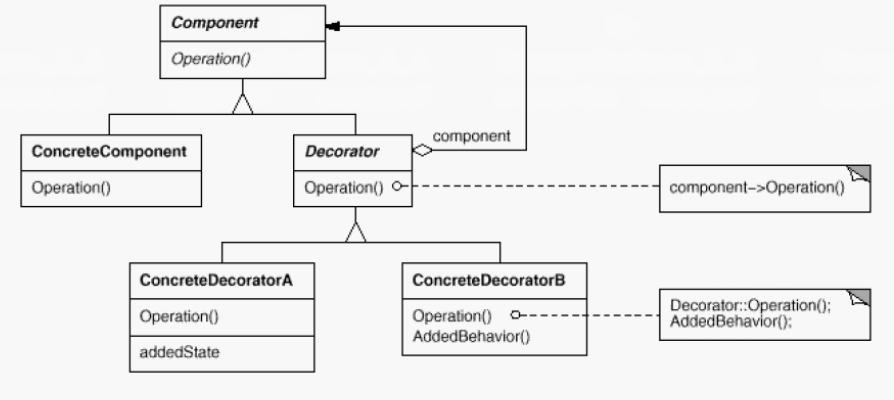
\includegraphics[width=0.7\linewidth]{Images/design_pattern/Decorator.png}
    \caption{Struttura del design pattern Decorator.}
\end{figure}

Dove:
\begin{itemize}
    \item \textbf{Component:} definisce l'interfaccia per gli oggetti a cui possono essere aggiunte responsabilità in modo dinamico.
    \item \textbf{ConcreteComponent:} definisce un oggetto al quale possono essere associate responsabilità aggiuntive.
    \item \textbf{Decorator:} mantiene un riferimento a un oggetto \textbf{Component} e definisce un'interfaccia che si conforma all'interfaccia del \textbf{Component}.
    \item \textbf{ConcreteDecorator:} aggiunge responsabilità al componente.
\end{itemize}


\newpage
\section{Factory Pattern}

\newpage
\section{Singleton Pattern}
Garantisce che una classe abbia una sola istanza e fornisce un punto di accesso globale ad essa. 

\begin{defn}[Continuity]
A function $f$ is continuous at $a$ if $\lim_{x\to a} f(x) = f(a)$.
\end{defn}

\begin{ex}[Prova]
Prova.
\end{ex}